\documentclass{beamer}
\usepackage[utf8]{inputenc}

\usetheme{Madrid}
\usecolortheme{default}
\useinnertheme{circles}

\definecolor{Logo1}{rgb}{0.208, 0.2865, 0.373}
\definecolor{Logo2}{rgb}{0.000, 0.674, 0.863}

\setbeamercolor*{palette primary}{bg=Logo1, fg=white}
\setbeamercolor*{palette secondary}{bg=Logo2, fg=white}
\setbeamercolor*{palette tertiary}{bg=white, fg=Logo1}
\setbeamercolor*{palette quaternary}{bg=Logo1,fg=white}
\setbeamercolor{structure}{fg=Logo1} % itemize, enumerate, etc
\setbeamercolor{section in toc}{fg=Logo1} % TOC sections

\usepackage{graphicx,animate}
%------------------------------------------------------------
%This block of code defines the information to appear in the
%Title page
\title[Linear Algebra] %optional
{Computing Techniques of Determinants}

\subtitle{Lecture 9}

\author[11910803@mail.sustech.edu.cn] % (optional)
{
    Zhang Ce
}

\institute[] % (optional)
{
    Department of Electrical and Electronic Engineering\\
    Southern University of Science and Technology
}

\date[2021.11.23] % (optional)
{2021.11.23}


%End of title page configuration block
%------------------------------------------------------------



%------------------------------------------------------------
%The next block of commands puts the table of contents at the
%beginning of each section and highlights the current section:

\AtBeginSection[]
{
\begin{frame}
    \frametitle{Table of Contents}
    \tableofcontents[currentsection]
\end{frame}
}
%------------------------------------------------------------


\begin{document}

%The next statement creates the title page.
\frame{\titlepage}


%---------------------------------------------------------
%This block of code is for the table of contents after
%the title page
\begin{frame}
\frametitle{Table of Contents}
\tableofcontents
\end{frame}
%---------------------------------------------------------
\section{A Brief Review of Last Lecture}
\begin{frame}{Last Lecture, We Discuss\dots}
Four parts in last lecture:
    \begin{enumerate}
        \item Orthogonal Vector and Subspaces\\
        inner product (dot product), definition of orthogonality
        \item Projection onto Lines\\
        geometrical interpretation, projection matrix
        \item Least Squares\\
        geometrical view and general projection matrices
        \item Interesting Applications of Linear Algebra\\
        chemistry, circuit principles and computer vision
    \end{enumerate}

\end{frame}

\begin{frame}{Gram-Schmidt}
\textbf{Algorithm Summary:}

\vspace{3pt}
Gram's Part:
\begin{itemize}
    \item Accept $\mathbf{a}$ to the orthogonal vector set.
    \begin{equation*}
        \mathbf{A}=\mathbf{a}
    \end{equation*}
    \item Subtract $\mathbf{A}$ component from $\mathbf{b}$ and add to the orthogonal vector set.
    \begin{equation*}
        \mathbf{B}=\mathbf{b}-\frac{\mathbf{b}^T\mathbf{A}}{\mathbf{A}^T\mathbf{A}}\mathbf{A}
    \end{equation*}
\end{itemize}

Schmidt's Part:
\begin{itemize}
    \item Normalize the vectors in orthogonal vector set.
    \begin{equation*}
        \mathbf{A}=\frac{\mathbf{A}}{||\mathbf{A}||}, \mathbf{B}=\frac{\mathbf{B}}{||\mathbf{B}||}
    \end{equation*}
\end{itemize}
\end{frame}














\section{Orthonormal Vectors and Orthogonal Matrices}
\begin{frame}{Orthonormal Vectors}
\begin{definition}
    The vectors $q_1,q_2,\cdots,q_n$ are orthonormal if
    \begin{equation*}
        {q_i}^Tq_j=\begin{cases}
            0, if\,\,i\ne j\\
            1, if\,\,i=j\\
        \end{cases}
    \end{equation*}
\end{definition}

What are the properties of orthonormal vector set?
\begin{itemize}
    \item Any 2 vectors are orthogonal.
    \item Every vector has a length of 1.
\end{itemize}

Well, give me some orthogonal vector set in $\mathbb{R}^2$.

\vspace{3pt}
(You may want to say the standard basis, that's true definitely, can you find some others?)
\end{frame}

\begin{frame}{Orthogonal Matrices}
If you write the orthonormal vectors in the columns of a matrix (kind of familiar?) to form $Q$, any properties?

\vspace{3pt}
$Qx=0$ has only the zero solution! That is because the column vectors are independent (orthogonal is the maximum independent).

\vspace{3pt}
How can I express the property of orthonormal vector set in matrix language (Think about $Q^TQ$)?


\begin{equation*}
    \left[ \begin{matrix}
        -&		-&		{q_1}^T&		-&		-\\
        -&		-&		{q_2}^T&		-&		-\\
        &		&		\vdots&		&		\\
        &		&		\vdots&		&		\\
        -&		-&		{q_m}^T&		-&		-\\
    \end{matrix} \right] _{m\times n}\left[ \begin{matrix}
        |&		|&		&		&		|\\
        |&		|&		&		&		|\\
        q_1&		q_2&		\cdots&		\cdots&		q_m\\
        |&		|&		&		&		|\\
        |&		|&		&		&		|\\
    \end{matrix} \right] _{n\times m}=I _{m\times m}
\end{equation*}

Are $m,n$ need to be equal? No, but if they are equal, orthogonal matrix.

\vspace{3pt}
For orthogonal matrices, $Q^T=Q^{-1}$. (familiar?)
\end{frame}

\begin{frame}{Orthogonal Matrices}
Why we create $Q$ (not necessarily square)? How can it be related to the previous knowledge in this chapter?

\vspace{3pt}
We have learnt the matrix representation of projection onto $C(A)$:
\begin{equation*}
    P=A(A^TA)^{-1}A^T
\end{equation*}

If we write down the matrix representation of projection onto $C(Q)$:
\begin{equation*}
    P=Q(Q^TQ)^{-1}Q^T=QQ^T
\end{equation*}

\vspace{3pt}
Recall 2 properties for projection matrices. Check if $QQ^T$ satisfies them?

\vspace{3pt}
In Chapter 3.3 least-squares, if we change $A$ to $Q$, what will we get?
\begin{equation*}
    A^TA\hat{x}=A^Tb\Rightarrow \hat{x}=Q^Tb\Rightarrow \hat{x}_i={q_i}^Tb
\end{equation*}

Which shows us the projection of $b$ on the $i$-th basis of $C(Q)$ is just the inner product of $q_i$ and $b$, that is correct because $||q_i||=1$.
\end{frame}

\section{Gram-Schmidt and QR Decomposition}
\begin{frame}{Gram-Schmidt}
We have known that orthogonal matrices have those "good" properties, a natural thought is: can I generalize and use the properties for all matrices?

\vspace{3pt}
That is the same to ask: can I transform any linearly independent vector set to orthonormal vector set? Gram and Schmidt answer yes!

\vspace{3pt}
Everything is difficult if you don't choose an easy example to analyze... How about start with 2 non-orthogonal independent vectors in $\mathbb{R}^2$?

\begin{figure}
    \centering
    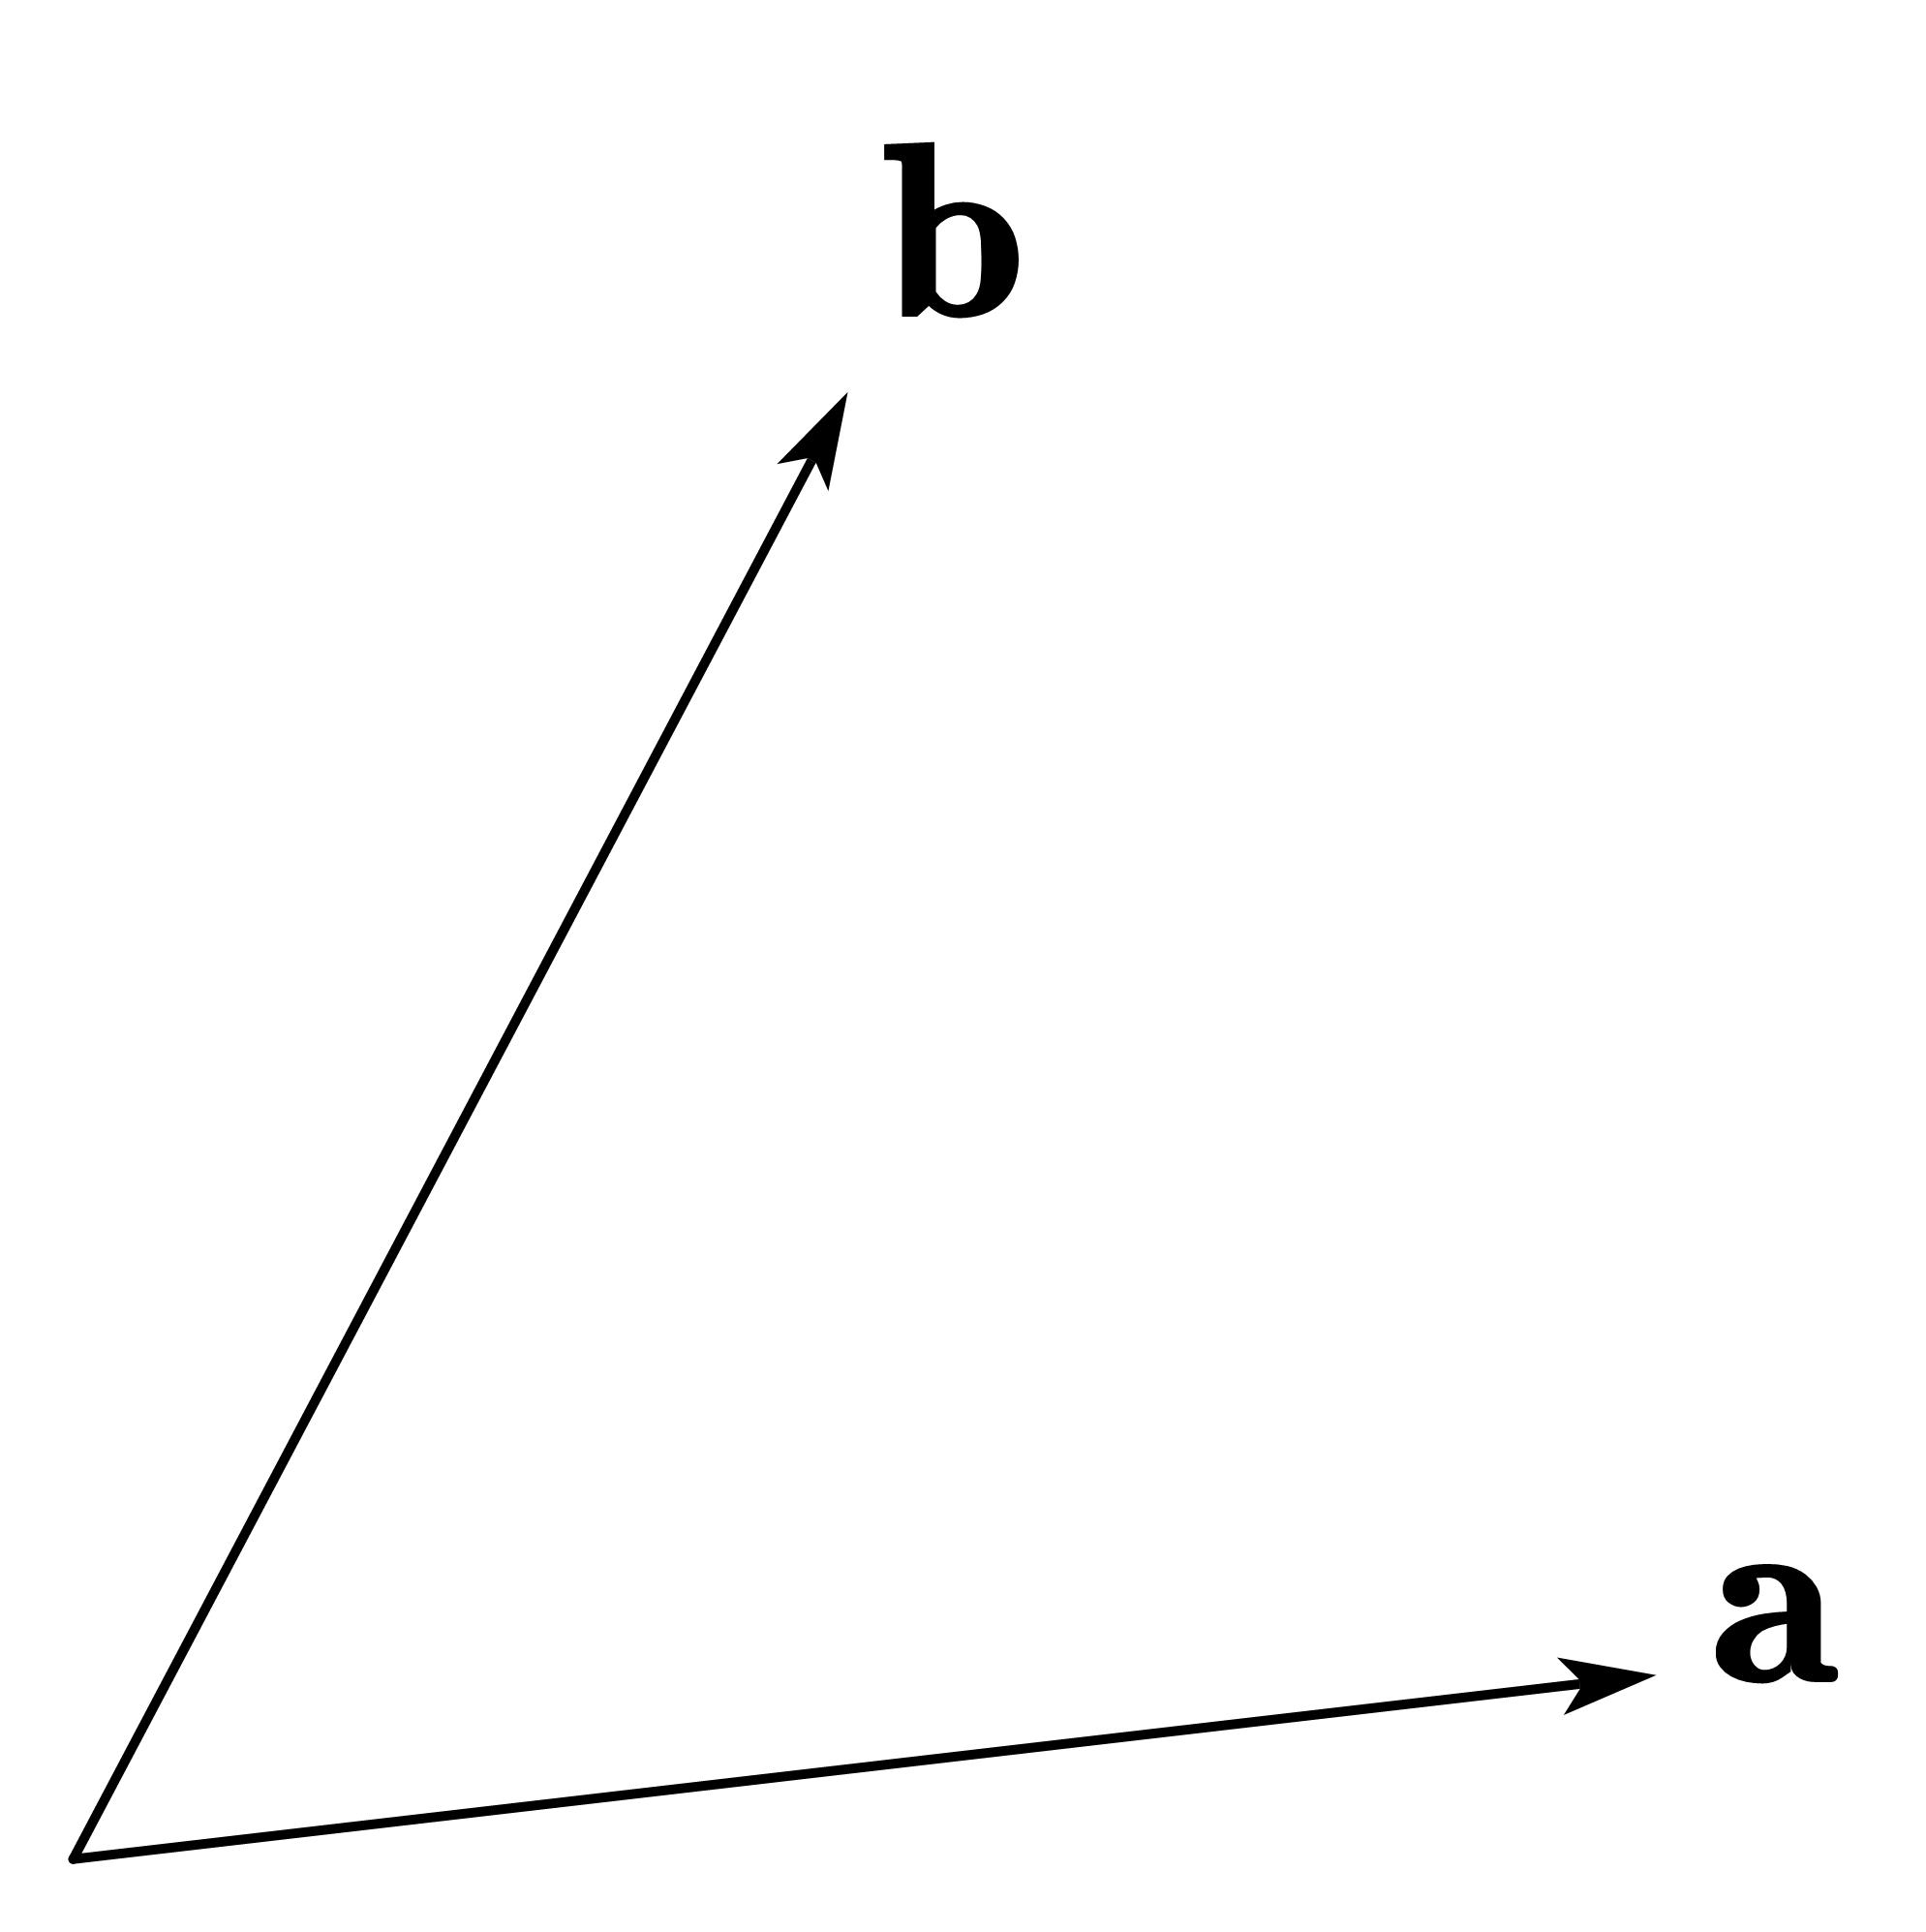
\includegraphics[width=0.3\textwidth]{gs.jpg}
\end{figure}

\end{frame}

\begin{frame}{Gram-Schmidt}
\begin{figure}
    \centering
    \includegraphics[width=1\textwidth]{gs1.jpg}
\end{figure}
\end{frame}

\begin{frame}{Gram-Schmidt}
\textbf{Algorithm Summary:}

\vspace{3pt}
Gram's Part:
\begin{itemize}
    \item Accept $\mathbf{a}$ to the orthogonal vector set.
    \begin{equation*}
        \mathbf{A}=\mathbf{a}
    \end{equation*}
    \item Subtract $\mathbf{A}$ component from $\mathbf{b}$ and add to the orthogonal vector set.
    \begin{equation*}
        \mathbf{B}=\mathbf{b}-\frac{\mathbf{b}^T\mathbf{A}}{\mathbf{A}^T\mathbf{A}}\mathbf{A}
    \end{equation*}
\end{itemize}

Schmidt's Part:
\begin{itemize}
    \item Normalize the vectors in orthogonal vector set.
    \begin{equation*}
        \mathbf{A}=\frac{\mathbf{A}}{||\mathbf{A}||}, \mathbf{B}=\frac{\mathbf{B}}{||\mathbf{B}||}
    \end{equation*}
\end{itemize}
\end{frame}

\begin{frame}{Gram-Schmidt}
\begin{example}
Do Gram-Schmidt orthogonalization for the vectors
\begin{equation*}
    \left[ \begin{array}{c}
        1\\
        1\\
        0\\
    \end{array} \right] , \left[ \begin{array}{c}
        1\\
        0\\
        1\\
    \end{array} \right] , \left[ \begin{array}{c}
        0\\
        1\\
        1\\
    \end{array} \right]
\end{equation*}
\end{example}
\textbf{Solution:}
Accept $\mathbf{a}$ to the orthogonal vector set:
\begin{equation*}
    a_1'=a_1=\left[ \begin{array}{c}
        0\\
        1\\
        1\\
    \end{array} \right]
\end{equation*}

Subtract $a_1'$ component from $a_2$ and add to the orthogonal vector set.
\begin{equation*}
    a_2'=a_2-\frac{a_2^Ta_1'}{a_1'^Ta_1'}a_1'=\left[ \begin{array}{c}
        0\\
        1\\
        1\\
    \end{array} \right] -\frac{1}{2}\left[ \begin{array}{c}
        1\\
        1\\
        0\\
    \end{array} \right] =\left[ \begin{array}{c}
        1/2\\
        -1/2\\
        1\\
    \end{array} \right]
\end{equation*}

\end{frame}

\begin{frame}{Gram-Schmidt}
Subtract $a_1'$ and $a_2'$ component from $a_3$ and add to the orthogonal vector set.
\begin{equation*}
    a_3'=a_3-\frac{a_3^Ta_1'}{a_1'^Ta_1'}a_1'-\frac{a_3^Ta_2'}{a_2'^Ta_2'}a_2'
\end{equation*}
\begin{equation*}
    =\left[ \begin{array}{c}
        0\\
        1\\
        1\\
    \end{array} \right] -\frac{1}{2}\left[ \begin{array}{c}
        1\\
        1\\
        0\\
    \end{array} \right] -\frac{1/2}{3/2}\left[ \begin{array}{c}
        1/2\\
        -1/2\\
        1\\
    \end{array} \right] =\left[ \begin{array}{c}
        -2/3\\
        2/3\\
        2/3\\
    \end{array} \right]
\end{equation*}

Finally, normalization:
\begin{equation*}
    q_1=\frac{1}{\sqrt{2}}\left[ \begin{array}{c}
        1\\
        1\\
        0\\
    \end{array} \right] , q_2=\frac{1}{\sqrt{6}}\left[ \begin{array}{c}
        1\\
        -1\\
        2\\
    \end{array} \right] , q_3=\frac{1}{\sqrt{3}}\left[ \begin{array}{c}
        -1\\
        1\\
        1\\
    \end{array} \right]
\end{equation*}
\end{frame}

\begin{frame}{QR Decomposition}
Experts in Linear Algebra will not stop here, they will go ahead to find the connection between $Q$ and $A$. That is the same with $LU$ decomposition, we find the matrix $L$ after we know how to find $U$. Now, we are going to find the connection $R$.

\begin{equation*}
    A=QR=\left( QQ^T \right) A\Rightarrow R=Q^TA
\end{equation*}
\begin{equation*}
    \left[ \begin{matrix}
        |&		|&		|\\
        a&		b&		c\\
        |&		|&		|\\
    \end{matrix} \right] =\left[ \begin{matrix}
        |&		|&		|\\
        q_1&		q_2&		q_3\\
        |&		|&		|\\
    \end{matrix} \right] \left[ \begin{matrix}
        {q_1}^Ta&		{q_1}^Tb&		{q_1}^Tc\\
        {q_2}^Ta&		{q_2}^Tb&		{q_2}^Tc\\
        {q_3}^Ta&		{q_3}^Tb&		{q_3}^Tc\\
    \end{matrix} \right]
\end{equation*}

In the Gram-Schmidt process, we can guarantee that ${q_2}^Ta=0$, why?

\begin{equation*}
    \left[ \begin{matrix}
        |&		|&		|\\
        a&		b&		c\\
        |&		|&		|\\
    \end{matrix} \right] =\left[ \begin{matrix}
        |&		|&		|\\
        q_1&		q_2&		q_3\\
        |&		|&		|\\
    \end{matrix} \right] \left[ \begin{matrix}
        {q_1}^Ta&		{q_1}^Tb&		{q_1}^Tc\\
        0&		{q_2}^Tb&		{q_2}^Tc\\
        0&		0&		{q_3}^Tc\\
    \end{matrix} \right]
\end{equation*}

$R$ is upper triangular! QR decomposition complete. A little bit complex...
\end{frame}

\section{Introduction and Properties of Determinant}
\begin{frame}{Introduction}
At first, I don't want to show you complex computations. A question is: determinant expresses what properties of matrix? Recall that every matrix can be recognized as a linear transformation.

\vspace{3pt}
Follow my opinion, consider the following matrix:
\begin{equation*}
    A=\left[ \begin{matrix}
        4&		0\\
        0&		2\\
    \end{matrix} \right]
\end{equation*}

Imaging the linear transformation process of this matrix, it is a linear transformation that stretches the 2-D plane on x and y directions! Actually, as you may know, $det(A)=8$, which reflects the stretching extent of linear transformation. To say in another way, if we trace an square or any kind of shape during linear transformation, the area will be multiplied by 8 after linear transformation.

\vspace{3pt}
Video(3B1B): https://www.bilibili.com/video/BV1ys411472E?p=7

\end{frame}

\begin{frame}{Properties of Determinant}
Now, let's consider the following properties for determinants geometrically.
\begin{itemize}
    \item $\left| \begin{matrix}
        1&		0\\
        0&		1\\
    \end{matrix} \right|=1, \left| \begin{matrix}
        0&		1\\
        1&		0\\
    \end{matrix} \right|=-1$
    \item $\left| \begin{matrix}
        ta&		b\\
        tc&		d\\
    \end{matrix} \right|=t\left| \begin{matrix}
        a&		b\\
        c&		d\\
    \end{matrix} \right|$
    \item Linearly dependent columns make the determinant 0
    \item $\det U=\left| \begin{matrix}
        d_1&		\ast&		\ast&		\cdots&		\ast\\
        0&		d_2&		\ast&		\cdots&		\ast\\
        0&		0&		d_3&		\cdots&		\ast\\
        \vdots&		\vdots&		\vdots&		\ddots&		\ast\\
        0&		0&		0&		0&		d_n\\
    \end{matrix} \right|=d_1d_2d_3\cdots d_n$
    \item $\det AB=\left( \det A \right) \left( \det B \right)$
\end{itemize}

We know all of them without any kinds of computations!
\end{frame}

\begin{frame}{Computation of Determinant}
Important formula (don't ask why, just remember):
\begin{equation*}
    \left| \begin{matrix}
        a&		b\\
        c&		d\\
    \end{matrix} \right|=ad-bc
\end{equation*}
\begin{equation*}
    \left| \begin{matrix}
        a_{11}&		a_{12}&		a_{13}\\
        a_{21}&		a_{22}&		a_{23}\\
        a_{31}&		a_{32}&		a_{33}\\
    \end{matrix} \right|= \cdots too\:long
\end{equation*}

And cofactor expansion (by row):
\begin{equation*}
    \left| \begin{matrix}
        a_{11}&		a_{12}&		a_{13}\\
        a_{21}&		a_{22}&		a_{23}\\
        a_{31}&		a_{32}&		a_{33}\\
    \end{matrix} \right|=a_{11}\left| \begin{matrix}
        a_{22}&		a_{23}\\
        a_{32}&		a_{33}\\
    \end{matrix} \right|-a_{12}\left| \begin{matrix}
        a_{21}&		a_{23}\\
        a_{31}&		a_{33}\\
    \end{matrix} \right|+a_{13}\left| \begin{matrix}
        a_{21}&		a_{22}\\
        a_{31}&		a_{32}\\
    \end{matrix} \right|
\end{equation*}

You can also expand by column. Be careful with those signs.

\vspace{3pt}
We will get deeper in next lecture. Please understand the geometrical interpretation, that's enough for this lecture!
\end{frame}


\end{document}